 
\chapter{Desenvolvimento das arquiteturas propostas}
\label{cap5}



Após o levantamento e fichamento dos requisitos para execução dos testes sobre as arquiteturas Rudy, Salz e Willson,
é notório a necessidade de exemplificar o funcionamento destas arquiteturas para jogos \ac{mmorpg}.
Nesse sentido, o capítulo atual irá levantar as devidas considerações sobre o desenvolvimento prático destas arquiteturas.


Em específico, a arquitetura física utilizou o mesmo conjunto de computadores, utilizando a mesma topologia.
%
Este tópico será abordado neste capítulo com maior profundidade na Seção~\ref{sec:topologia}.
%
Em seguida, é relatado o funcionamento do sistema de coleta de informações de recursos, a qual será abordada a Seção~\ref{sec:informacoes}.

A explicação técnica dos projetos estão organizadas da seguinte forma para cada serviço desenvolvido das arquiteturas:


\begin{enumerate}
    \item Linguagem de Programação e bibliotecas: Exibe pontos a cerca das linaguagens de programação e quais módulos ou bibliotecas foram utilizados para o seu desenvolvimento.
    \item Protocolos Utilizados: Mostra quais protocolos estes serviços utilizam para troca de mensagens em seu ecossistema. Será mostrado utilizando uma tabela de adjacência, tal qual utilizado para relação entre nós em um Grafo.
    \item Processamento ativo interno: Demonstra qual o processamento ativo no serviço independente das requisições de seus microsserviços vizinhos ou cliente.
\end{enumerate}



Ao final será levantado o funcionamento do cliente das arquiteturas Rudy (Subseção \ref{rudy}), Salz (Subseção \ref{salz}) e Willson (Subseção \ref{willson}).
%
Nesta etapa será exibido o fluxo de mensagens a partir das ações realizadas pelo cliente.
%
Nesse sentido este capítulo deve abrangir todos os aspéctos técnicos da aplicação, levando em consideração o seu fluxo de funcionamento e integração entre os microsserviços no ecossistema da arquitetura.


\section{Topologia da Rede}
\label{sec:topologia}

A topologia da rede segue o padrão proposto para a coleta de dados.
%
O seu principal objetivo é segregar as instâncias na camada de rede, evitando interferências do orquestrador de microsserviços que será utilizado na implantação.
%
Por muitas vezes, a fim de otimizar o transporte de dados, estes orquestradores trocam mensagens na rede utilizando memória, visto que uma conexão pode ser realizada para a máquina do próprio hospedeiro.
%
Segregando em regiões, o orquestrador será forçado a realizar a conexão com as instâncias externas, forçando a utilização da pilha completa do protocolo \ac{tcp} e \ac{udp}.

Para realizar esta divisão, foi utilizado o gestor da Núvem Tchê, orquestrada com o OpenStack.
%
A topologia utilizada nos testes com as três arquiteturas podem ser visualizada na Figura~\ref{fig:topologia}.

\begin{figure}[htb!]
    \caption{Topologia de Rede}
    \label{fig:topologia}
    \begin{minipage}{.45\textwidth}
        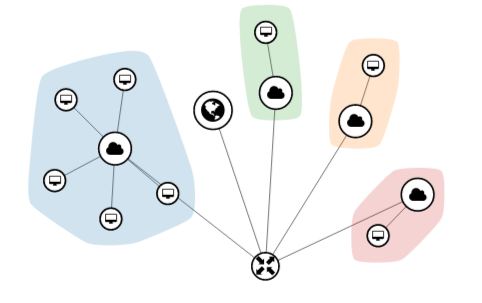
\includegraphics[height=5.5cm]{img/cap5/topology_graph.png}
      \centering
    \end{minipage}
    \begin{minipage}{.45\textwidth}
        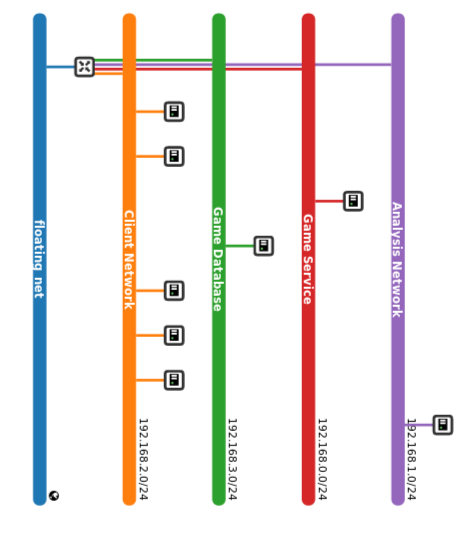
\includegraphics[height=6.5cm]{img/cap5/topology.png}
        \centering        
    \end{minipage}


    Fonte: O próprio Autor.
\end{figure}

A Figura~\ref{fig:topologia} mostra a disposição das instâncias em sub-redes exibindo-as em formato de árvore e em barras.
%
A visualização com formato árvore ajuda a compreender a conexão entre cada máquina do ambiente de testes.
%
Já a visualização em formato barra, exibe características técnicas como a divisão por \ac{ip} e nome da rede.
%
Ambos os gráficos são complementares para formar as características básicas da interconexão das sub-redes.

A Figura~\ref{fig:topologia} também exibe 8 instâncias utilizadas nos testes.
%
Cada instância pode ter configurações padrões de \ac{os}, \acs{vcpu}, memória.
%
Além disso, o OpenStack permite a criação rápida de réplicas de uma instância.
%
Dessa forma facilitando a configuração da rede final.
%
As características específicas das instâncias podem ser visualizados na Tabela~\ref{tab:instancias}.

\begin{table}[htb!]
    \centering
    \caption{Instâncias das redes de teste}
    \label{tab:instancias}
    \begin{tabular}{|l|l|l|l|l|l|}
        \hline
        Nome                                                              & \ac{os}             &\acs{vcpu}& Memória & Rede ou IP   & Réplicas \\ \hline
        \begin{tabular}[c]{@{}l@{}}client\_one\\ client\_two\end{tabular} & Ubuntu Server 16.04 & 1        & 1 GB    & 192.168.2.*  & 5        \\ \hline
        game\_service                                                     & Ubuntu Server 16.04 & 4        & 8 GB    & 192.168.0.8  & 1        \\ \hline
        game\_database                                                    & Ubuntu Server 16.04 & 1        & 1 GB    & 192.168.3.11 & 1        \\ \hline
        data\_analisys                                                    & Ubuntu Server 16.04 & 4        & 4 GB    & 192.168.1.2  & 1        \\ \hline
    \end{tabular}

    Fonte: O próprio Autor.
\end{table}

A Tabela~\ref{tab:instancias} exibe as configurações exatas utilizadas nos testes.
%
As instâncias \textit{client\_one} e \textit{client\_two} são responsáveis por executar os clientes a qual realizam o ataque de carga ao serviço.
%
A instância \textit{game\_service} é responsável unicamente por executar os microsserviços das arquiteturas Rudy, Salz e/ou Willson.
%
A instância \textit{game\_database} é responsável por executar o banco de dados Postgres e Redis, ambos utilizados em todas as arquiteturas.
%
Por fim, a instância \textit{data\_analisys} é responsável por executar o banco de métricas e o sistema de monitoramento.

A gestão das instâncias, dentro de cada sub-rede, foi automatizado com algum sistema de orquestração de microsserviços, em nível de aplicação.
%
Nesse sentido, a configuração inicial de cada instância foi feita de forma automatizada, com um script na linguagem \textit{Bash} na qual configurava o ambiente com a plataforma \textit{Docker}.
%
A Tabela~\ref{tab:docker_versoes} mostra detalhes sobre as versões do Docker instalados na máquina e o orquestrador escolhido para operação.

\begin{table}[htb!]
    \centering
    \caption{Orquestradores utilizados no teste.}
    \label{tab:docker_versoes}
    \begin{tabular}{|l|l|l|l|}
    \hline
        Nome                                                              & Docker Engine & Docker Compose & Orquestrador   \\ \hline
        \begin{tabular}[c]{@{}l@{}}client\_one\\ client\_two\end{tabular} & 18.09         & 3.0            & Docker Swarm   \\ \hline
        game\_service                                                     & 18.09         & 3.0            & Docker Swarm   \\ \hline
        game\_database                                                    & 18.09         & 3.0            & Docker Compose \\ \hline
        data\_analisys                                                    & 18.09         & 3.0            & Docker Compose \\ \hline
    \end{tabular}

    Fonte: O próprio Autor.
\end{table}

Em específico neste projeto, foram utilizados os orquestradores Docker Swarm e Docker Compose, como visível na Tabela~\ref{tab:docker_versoes}.
%
Estes dois orquestradores facilitam, respectivamente, a implantação de arquiteturas complexas sem relacionamento com o disco rígido e o controle de volumes para armazenamento temporário de dados.
%
Dessa forma, os serviços implantados nas instâncias \textit{game\_service} e \textit{client\_*} são gerenciados pelo Docker Swarm, visto que ambos não necessitam de acesso a disco e podem ser escalados para mais de uma instância.
%
Por sua vez, os serviços restantes precisam de acesso a disco. Dessa forma eles foram implantados utilizando o Docker Compose.


Em especial, sistema de coleta de métricas é executado na instância \textit{data\_analisys} e foi implantado utilizando Docker Compose. Esta instância é uma peça fundamental para o sucesso do atual trabalho, haja vista que toda a captura de métricas será armazenada e processada por esta instância.
%
Nesse sentido, faz-se necessário detalhar o funcionamento deste sistema computacional.


\section{Sistema de coleta de informações de recursos}
\label{sec:informacoes}

O sistema de coleta de informações tem como principal objetivo receber requisições do estado da aplicação ou instância.
%
Em específico para esta aplicação, o sistema de métricas relacionará um montante (GBs, MBs, Tempo de Requisição) em relação ao tempo, formando assim gráficos a qual podem ser comparados entre sí dentro de um período.

Para esta solução, a pilha de monitoramento escolhida é o banco de dados para métricas Graphite e o gestor web para visualização Grafana.
%
Estas soluções foram escolhidas por afinidade, facilidade de uso e por serem ferramentas de uso em ambientes reais para este objetivo.
%
A aplicação Grafana pode ser visualizada na Figura~\ref{fig:grafana}.


\begin{figure}[htb!]
    \caption{Captura de recursos utilizando Grafana}
    \label{fig:grafana}
    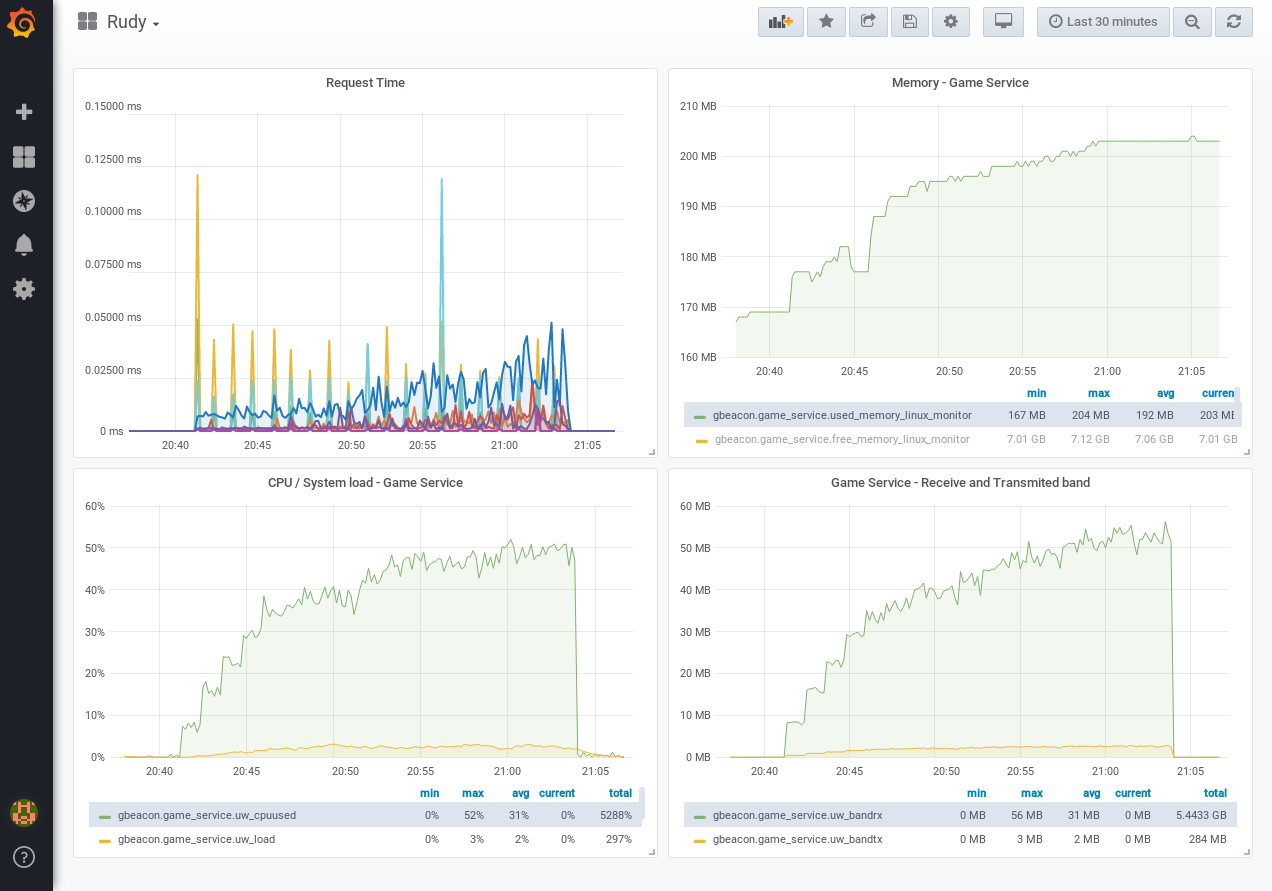
\includegraphics[height=7.0cm]{img/cap5/web.png}
    \centering

    Fonte: O próprio Autor.
\end{figure}

Utilizando o Grafana, é possível verificar e comparar períodos diretamente por seu sistema web, durante a execução dos testes.
%
Isto permite maior flexibilidade e segurança da obtenção de dados, na qual são monitorados de forma facilitada pelo operador dos testes em seu painel de operações, como exibido na Figura~\ref{fig:grafana}.

O Grafana exibirá os dados armazenados no banco de dados Graphite.
%
Este banco de dados é específico para armazenamento de métricas.
%
Nesse sentido, ele é capaz de otimizar a transferência de informações a qual são enviadas do serviço de jogo e do cliente.

Existem dois tipos de clientes a qual populam os dados automaticamente no sistema de monitoramento.
%
O cliente de recurso e cliente de tempo. O Cliente de recurso será utilizado no \textit{game\_service} na qual enviará métricas do consumo de recursos pela instância.
%
Além deste, o cliente de tempo é responsável por popular dados referente ao tempo que levará para executar cada requisição ao serviço, executado no \textit{game\_client}.

Os dados serão analisados tanto nos gráficos padrões de monitoramento do grafana, quanto utilizando dos dados brutos, na qual são obtidos através da \ac{api} de render do Graphite.
%
Nesse sentido, também será dado a flexibilidade de obter métricas para estudos estatísticos externos a pilha padrão.

\section{Arquitetura Rudy}
\label{sec:arc_rudy}

A arquitetura Rudy (Subseção \ref{rudy}), a primeira arquitetura a ser desenvolvida, teve o seu funcionamento reduzido aos microsserviços básicos para o funcionamento do Gerente de Mundo.
%
Nesse sentido, os microsserviços implementados para esta arquitetura foram:

\begin{enumerate}
    \item Serviço de Jogo: Ou \textit{rudygh}.
    \item Gerenciador de Consultas: Ou \textit{rudydb}.
    \item Serviço de Autenticação: Ou \textit{rudya}.
    \item Serviço Web Dinâmico: Ou \textit{rudyweb}.
\end{enumerate}



Além destes microsserviços, a arquitetura utiliza os serviços PostgreSQL e Redis, ambas de código aberto.
%
Tais serviços são utilizados respectivamente como banco de dados permanente e banco de dados em memória cache para autenticação.
%
Este método de autenticação foi replicado para as demais arquiteturas.



Em relação aos protocolos utilizados na arquitetura Rudy, temos dois serviços RPC e dois serviços HTTP.
%
A relação detalhada é exibida na Tabela~\ref{tab:protocolos_rudy}.



\begin{table}[htb!]
    \centering
    \caption{Protocolos dos microsserviços da arquitetura Rudy.}
    \label{tab:protocolos_rudy}
    \begin{tabular}{|l|l|l|l|}
    \hline
    Microsserviço & Linguagem de Programação    & Porta & Protocolo \\ \hline
    rudygh        & Golang 1.11 / RPC Nativo    & 3000  & TCP       \\ \hline
    rudydb        & Golang 1.11 / Gin Framework & 3000  & HTTP      \\ \hline
    rudya         & Golang 1.11 / RPC Nativo    & 3000  & TCP       \\ \hline
    rudyweb       & Golang 1.11 / Gin Framework & 3000  & HTTP      \\ \hline
    \end{tabular}
    
    Fonte: O próprio autor.
\end{table}

Além de quais protocolos, a Tabela~\ref{tab:protocolos_rudy} exibe qual tecnologia está utilizando para manter o serviço.
%
Tanto nos microsserviços da arquitetura Rudy quanto aos demais microsserviços implementados para este TCC foram escritos na linguagem Go.
%
Ambos os serviços compartilham dos mesmos modelos de padrão \ac{mvc} tanto para as aplicações \ac{rpc} e \ac{http}.

Para o desenvolvimento dos microsserviços da arquitetura Rudy, foram utilizados os seguintes pacotes externos da linguagem:

\begin{itemize}
    \item Gin: Framework focado em desenvolvimentos de \ac{api} para web escrito em Golang.
    \item Redis: Pacote de conexão sobre \ac{tcp} ou \ac{udp} em um serviço Redis.
    \item Protofub: Pacote que implementa serialização de dados estruturados de modo mínimo. É utilizado para minimizar custo de chamadas \ac{rpc} em Go.
    \item Gorm: Golang \ac{orm} que permite a conexão com o banco de dados Postgres sem utilizar \ac{sql}.
    \item Graphite: Pacote que permite a conexão com o servidor de logs Graphite para enviar métricas.
    \item Gorequest: Pacote para estruturar requisições Web utilizado para comunicação interna entre serviços Web utilizando assinatura \ac{jwt}.
    \item Testify: Suíte de testes para manter o funcionamento íntegro durante a implementação da aplicação. Em específico, a aplicação possúi 90\% de convergência de código, a qual garante a integridade de futuras alterações.
\end{itemize}

Todas as bibliotecas utilizadas são distribuídas com modelo \it{Open Source}, pelas licenças \it{MIT}, \it{BSD} e \it{GPLv3}.
%
Estas mesmas bibliotecas são utilizadas nas demais arquiteturas.